\chapter{Implementación}

\section{Implementación de la Vista}

\subsection{Herramientas para el desarrollo}

Para la programación del sitio web se ha hecho uso de los lenguajes de programación HTML, CSS, y Javascript. En concreto, se ha utilizado HTML5 y CSS3.

Adicionalmente, se han empleado recursos varios, como pueden ser imágenes extraídas de Internet y un plugin para la creación de ventanas emergente, SweetAlert2 \footnote{\url{https://sweetalert2.github.io}}. En concreto, este plugin lo forman dos archivos extraídos del repositorio de la aplicación en JSDelivr \footnote{\url{https://www.jsdelivr.com/package/npm/sweetalert2}}. Como se puede ver en esta página, la versión empleada de SweetAlert2 es 11.4.17. Los dos archivos se guardan una carpeta concreta llamada plugin que se encuentra junto a la carpeta de imágenes y la carpeta de scripts de Javascript.

\subsection{Interfaz responsive}

Una interfaz responsive es un tipo de interfaz que se adapta al dispositivo donde se esté visualizando el sitio web. Para conseguir esta adaptación se hace uso de una cierta estructura del lenguaje CSS. Esta estructura son los @media. Dentro de esta estructura se puede indicar que restricciones queremos que se cumplan sobre la pantalla, como pueden ser el máximo y el mínimo, tanto de ancho como de alto de la pantalla. Con estas restricciones se van generando los estilos propios de cada dispositivo.

Las restricciones que se han utilizado son las mostradas en la Tabla \ref{tab:restri_tam_dispo}.

\begin{table}[h]
\centering
\resizebox{\textwidth}{!}{%
\begin{tabular}{c|cc|cc|}
\cline{2-5}
\multicolumn{1}{l|}{} &
  \multicolumn{2}{c|}{\cellcolor[HTML]{FFFC9E}\textbf{Altura}} &
  \multicolumn{2}{c|}{\cellcolor[HTML]{FFFC9E}\textbf{Anchura}} \\ \cline{2-5} 
\multicolumn{1}{l|}{} &
  \multicolumn{1}{c|}{\cellcolor[HTML]{FFCE93}\textbf{Max.}} &
  \cellcolor[HTML]{FFCE93}\textbf{Min.} &
  \multicolumn{1}{c|}{\cellcolor[HTML]{FFCE93}\textbf{Max.}} &
  \cellcolor[HTML]{FFCE93}\textbf{Min.} \\ \hline
\multicolumn{1}{|c|}{\cellcolor[HTML]{FFFC9E}\textbf{Portátil}} &
  \multicolumn{1}{c|}{1080px} &
  751px &
  \multicolumn{1}{c|}{1920px} &
  1025px \\ \hline
\multicolumn{1}{|c|}{\cellcolor[HTML]{FFFC9E}\textbf{Tablet Horizontal}} &
  \multicolumn{1}{c|}{750px} &
  500px &
  \multicolumn{1}{c|}{1024px} &
  751px \\ \hline
\multicolumn{1}{|c|}{\cellcolor[HTML]{FFFC9E}\textbf{Tablet Vertical}} &
  \multicolumn{1}{c|}{1024px} &
  751px &
  \multicolumn{1}{c|}{750px} &
  500px \\ \hline
\multicolumn{1}{|c|}{\cellcolor[HTML]{FFFC9E}\textbf{Móvil}} &
  \multicolumn{1}{c|}{850px} &
  500px &
  \multicolumn{1}{c|}{400px} &
  200px \\ \hline
\end{tabular}%
}
\caption{Restricciones de tamaño de pantalla para los dispositivos}
\label{tab:restri_tam_dispo}
\end{table}

Para obtener estas medidas de pantalla se han analizado varios dispositivos de cada uno de los tipos de dispositivo utilizados en la Tabla \ref{tab:restri_tam_dispo}.

Un caso de uso de distintos estilos según el dispositivo, es la visualización de la descripción de la página principal y del mockup. Cuando el dispositivo tiene la suficiente anchura, se muestran ambos elementos en paralelo, como se puede ver en la Figura \ref{fig:responsive_portatil} (Portátil, Tablet Horizontal); mientras que cuando la anchura no lo permite, se muestran uno detrás del otro como se puede ver en la Figura \ref{fig:responsive_tablet} (Tablet Vertical, Móvil).

\begin{figure}[H]
\centering
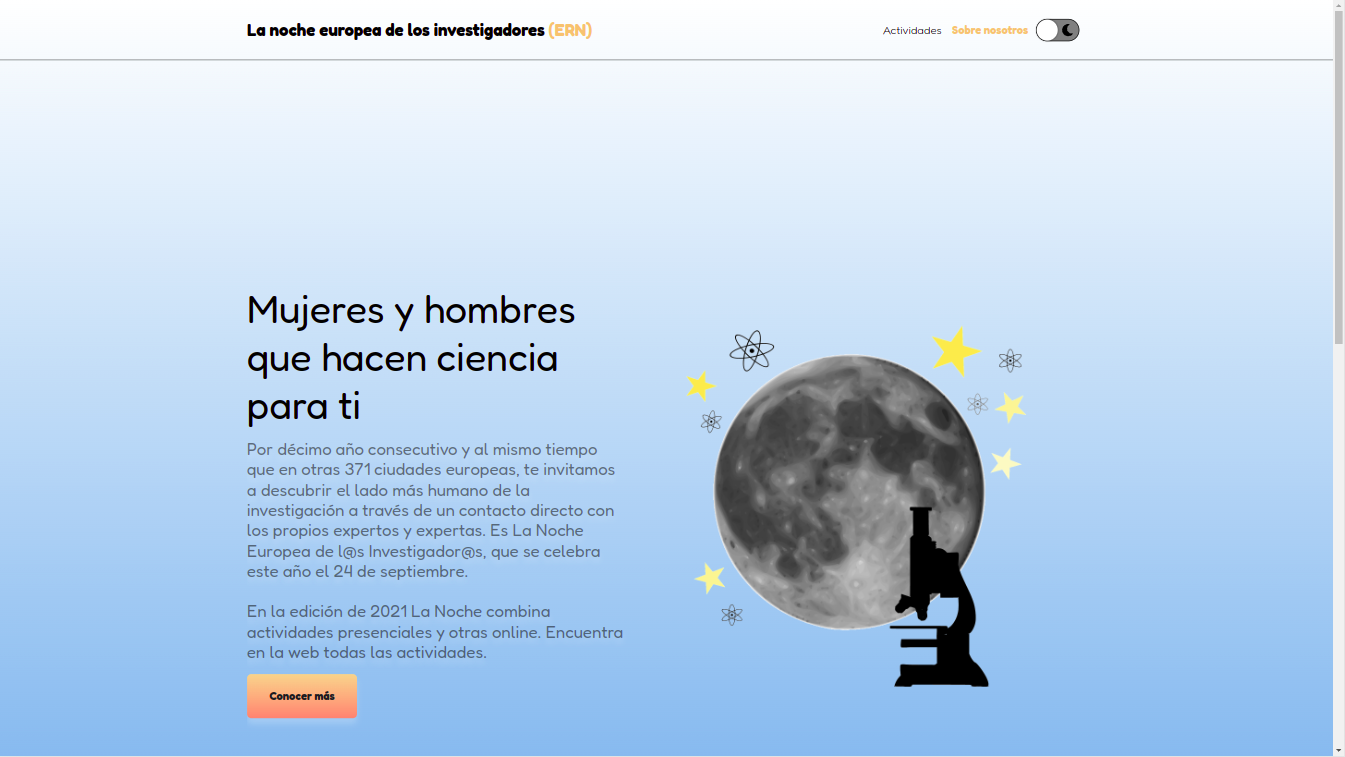
\includegraphics[width=0.8\textwidth]{imagenes/07_Implementacion/responsive_portatil.png}
\caption{Interfaz responsive usando el portátil}
\label{fig:responsive_portatil}
\end{figure}

\begin{figure}[H]
\centering
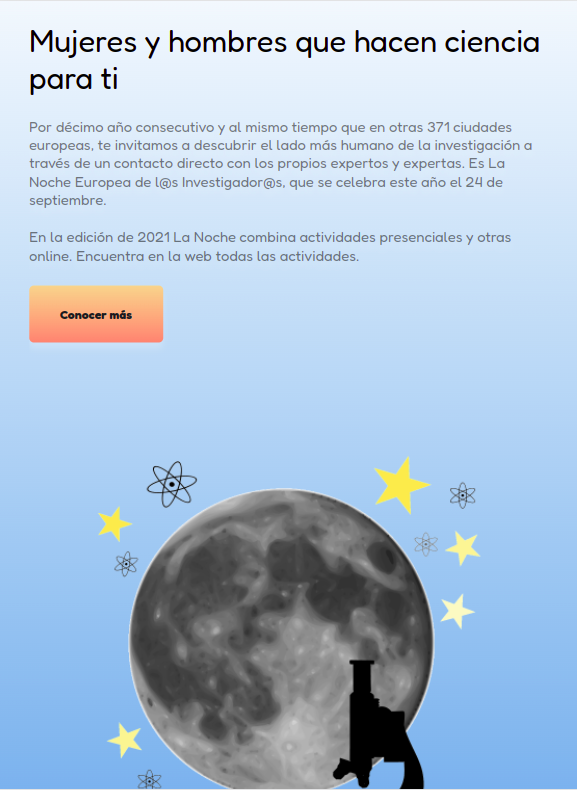
\includegraphics[width=0.6\textwidth]{imagenes/07_Implementacion/responsive_tablet.png}
\caption{Interfaz responsive usando la tablet en orientación vertical}
\label{fig:responsive_tablet}
\end{figure}

Esta filosofía de creación de sitios web permite crear varios sitios web definiendo una única vez los elementos que forman el sitio web y definiendo varios estilos que modifiquen los atributos de esos elementos.

\subsection{Modo oscuro}

Una vez hemos generado el tema claro del sitio web, será necesario implementar los elementos que hacer funcionar este cambio de tema. Para ello será necesario implementar un interruptor para cambiar de tema en cualquiera de las secciones del sitio web y por último elaborar los estilos para el modo oscuro.

Para generar el interruptor será necesario crear un elemento nuevo en la barra de navegación de las distintas secciones del sitio web. El interruptor será un elemento compuesto por dos espacios, donde en cada espacio habrá un icono de un sol y una luna respectivamente; y una bola que se encuentra en el interior de estos dos espacios y que se desplaza del extremo izquierdo al extremo derecho y viceversa.

Una vez definidos los componentes de este interruptor es hora de explicar como se ha implementado el movimiento del interruptor para cambiar de tema. Este movimiento se simula a través del cambio del estilo del interruptor. En un principio el interruptor tiene el estilo \textit{switch\_dark\_mode}, el cual coloca la bola de su interior en el extremo izquierdo, dejando ver el icono de la luna. De esta forma estamos indicando que al hacer clic en el interruptor se pasará al modo oscuro que está asociado con el icono de la luna. Dentro del estilo \textit{switch\_dark\_mode} se definen todos los atributos del espacio que ocupa el interruptor, ya que los atributos de la bola se definen en la parte \textit{::after} del estilo \textit{switch\_dark\_mode}. Los atributos de la bola se definen en esta sección porque se trata de un pseudo-elemento del interruptor. Hasta ahora tendremos los estilos del interruptor cuando está inactivo y, por lo tanto, el sitio web se encuentra en el tema claro. Falta definir los atributos que cambiaran del estilo del interruptor al activar el interruptor. Para tener de base los atributos del interruptor en modo inactivo y solamente tener que modificar el color y la posición de la bola al activar el interruptor, se añadirá o eliminará el estilo \textit{active} al estilo \textit{switch\_dark\_mode}. En este nuevo estilo \textit{active} se indica cuál será el color del interruptor cuando se encuentra activo y sitúa la bola en el extremo derecho del interruptor, dejando ver el icono del sol, el cual está asociado con el modo claro y, por lo tanto, indicando que si se vuelve a pulsar sobre el interruptor se desactivará el interruptor y se volverá al modo claro.

Visualmente, el estado del interruptor se muestra distinto en modo inactivo (
\includegraphics[width=0.07\textwidth]{imagenes/07_Implementacion/switch_inactive.png}) que en modo activo (
\includegraphics[width=0.07\textwidth]{imagenes/07_Implementacion/switch_active.png}).

Por último, falta implementar la parte dinámica de este interruptor, ya que hasta ahora únicamente hemos definido los elementos y los estilos que forman el interruptor, pero es necesario que el cambio de estilos del interruptor se realice mientras se utiliza el sitio web. Para implementar esta funcionalidad se crea un script de Javascript, el cual es incluido en todas las secciones del sitio web para poder hacer uso del interruptor en cada una de ellas. Dentro de este script se obtiene el elemento HTML que contiene al interruptor y posteriormente se define un evento de clic al pulsar sobre el interruptor. Al definir este evento, asignamos la ejecución de una función al hacer clic sobre el interruptor. La función a ejecutar consiste en dos comandos toggle. Lo que hace un comando toggle en Javascript es añadir el estilo que se le indica, al elemento sobre el que se ejecuta el comando; o eliminar el estilo si el elemento sobre el que se ejecuta el comando ya contiene el estilo. En primer lugar, se añade o elimina el estilo \textit{dark\_mode} a todos los elementos de la página web. Y en segundo punto, se añade o elimina el estilo \textit{active} al interruptor.

Ya solamente necesitamos crear los estilos \textit{dark\_mode} de cada uno de los elementos en los que sea necesario cambiar su color al cambiar a modo oscuro.

\subsection{Menú lateral}

Para la implementación de esta funcionalidad serán necesarios dos elementos. Por un lado, el botón para desplegar el menú; y, por otro lado, el propio menú lateral.

El botón para desplegar el menú consiste en un simple botón de HTML, al cual se le añade un icono (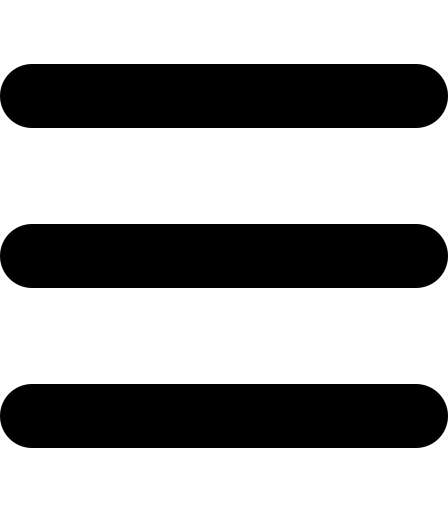
\includegraphics[width=0.03\textwidth]{imagenes/07_Implementacion/bars-solid.png}).

Para implementar el despliegue y la ocultación del menú lateral se hace uso de la misma táctica que con el interruptor para el cambio de tema de colores. Esta táctica consiste en utilizar distintos estilos para variar la apariencia de los elementos que deseamos. Siguiendo esta táctica se creará el estilo \textit{sidebar}, que afecta al menú lateral. Este primer estilo mantiene oculto al menú lateral. En segundo lugar, se genera el estilo \textit{deploy}, que también afecta al menú lateral, y el cual hace visible al menú lateral. Con estos dos estilos podemos implementar la funcionalidad del menú lateral.

Para implementar la funcionalidad se hace empleo de un script de Javascript, el cual se coloca en todas las secciones del sitio web, al igual que se hace con el script para el interruptor. Dentro de este script se obtiene tanto el botón de despliegue como el elemento que contiene al menú lateral. Por último, asignaremos un evento de clic al botón obtenido. Al pulsar el botón se ejecutará una función que añadirá o eliminará el estilo deploy del menú lateral, haciendo visible o no visible respectivamente al menú lateral.

Un ejemplo de los dos estados que puede tener el menú lateral se pueden ver en la Figura \ref{subfig:menu_oculto}, donde se puede ver el menú lateral oculto; y en la Figura \ref{subfig:menu_desplegado}, donde se puede ver el menú lateral despegado.

\begin{figure}[h]
\centering
\subfloat[Estado oculto]{
\label{subfig:menu_oculto}
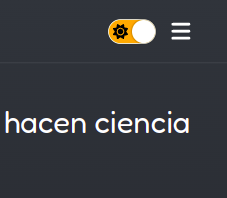
\includegraphics[width=0.3\textwidth]{imagenes/07_Implementacion/menu_oculto.png}}
\subfloat[Estado desplegado]{
\label{subfig:menu_desplegado}
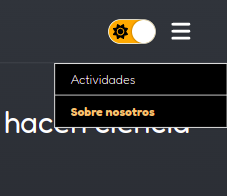
\includegraphics[width=0.3\textwidth]{imagenes/07_Implementacion/menu_desplegado.png}}
\caption{Estados del menú lateral}
\label{fig:estados_menu_lateral}
\end{figure}

\subsection{Ventanas emergentes}

El lenguaje Javascript tiene por defecto órdenes para crear ventanas emergentes, pero estas ventanas tienen un estilo muy básico. Para tener ventanas emergentes con un estilo interesante para el usuario se ha utilizado el plugin SweetAlert2. En su página oficial \footnote{\url{https://sweetalert2.github.io}} se muestran varios ejemplos de usos de este plugin. Para la creación de mis ventanas me he basado en varios de estos ejemplos. Para empezar a poder usar este plugin es necesario incluir en el archivo HTML de la página donde se quiera usar, un enlace a los archivos que forman el plugin.

Todas las ventanas disponen de una serie de atributos \footnote{\url{https://sweetalert2.github.io/#title}}, los cuales pueden ser definidos o no. Entre ellos podemos encontrar el título de la ventana, el color de los botones, y muchos más.

Para lanzar la ventana y que se haga visible, se emplea la función \textit{Swal.fire}\ . Pero aquí no queda la cosa porque existen ventanas que dan solamente información, y otras que dan información y esperan una interacción del usuario; lo interesante de estas últimas es que se debe gestionar la respuesta del usuario. Esta gestión se realiza en el \textit{then} de la función \textit{Swal.fire}, el cual se activa cuando esta función devuelve una \textit{Promise}.

La información que se suele gestionar es la indicación de que botón ha pulsado el usuario. Para ello, este plugin dispone de funciones que nos facilitan conocer esta información, las cuales se pueden comprobar en su página oficial en el apartado "Handling buttons".

Hasta este momento se puede tener una idea de como funcionan estas ventanas emergentes. Falta explicar como las hemos utilizado en nuestro sistema. En nuestro caso hemos creado tres ventanas emergentes distintas. Todas las ventanas originadas hacen uso del botón de confirmación y de cancelación. Estas ventanas se describen a continuación:

\begin{itemize}
\item \textbf{Permiso para la toma de imágenes:} Esta ventana se lanza al pulsar sobre alguno de los botones que abre el chatbot en alguno de los canales disponibles. Estos botones se pueden ver en la Figura \ref{fig:botones_canales}.

\begin{figure}[h]
\centering
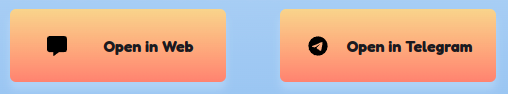
\includegraphics[width=0.7\textwidth]{imagenes/07_Implementacion/botones_canales.png}
\caption{Botones para el acceso a los canales de comunicación con el chatbot}
\label{fig:botones_canales}
\end{figure}

La ventana emergente informa al usuario de que la deducción de la edad se va a producir a través de una imagen, y, por lo tanto, si quiere o no que se le tomen imágenes. Además, se indica que no se puede revertir la decisión. Esta ventana se puede ver en la Figura \ref{fig:popup_pemisos}.

En el caso de que el usuario confirme la toma de imágenes, se abrirá la sección de captura de imágenes. En caso contrario, al negar la toma de imágenes por parte del usuario se lanzará una nueva ventana emergente.

\item \textbf{Indicación explícita de la edad:} Esta ventana emergente es la que se genera en caso de negar la toma de imágenes en la ventana emergente del punto anterior. En esta ventana se preguntará explícitamente la edad del usuario. Y además, aparecerán exactamente dos rangos de edad: Niño o Adulto. Esta ventana se puede ver en la Figura \ref{fig:popup_edad}. Cuando el usuario elige alguno de los dos rangos de edad, se abrirá la interfaz del chatbot a través del canal que haya elegido el usuario cuando pulsó el botón que lanzó la primera ventana emergente.

\begin{figure}
    \centering
    \subfloat[Ventana emergente para la adquisición de permisos de toma de imágenes]{
    \begin{subfigure}
        \centering
        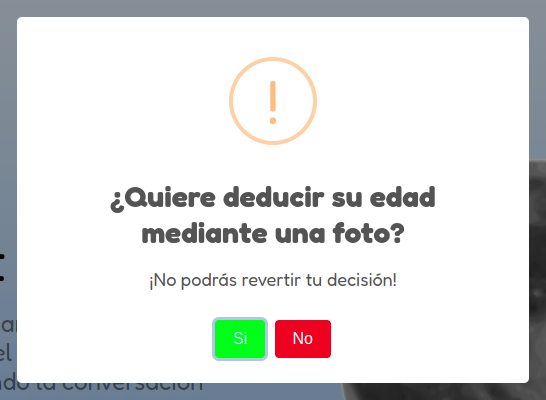
\includegraphics[width=0.4\textwidth]{imagenes/07_Implementacion/popup_permisos.png}
        \label{fig:popup_pemisos}
    \end{subfigure}
    }
    \hspace{5mm}
    \subfloat[Ventana emergente para la deducción de la edad]{
    \begin{subfigure}
        \centering
        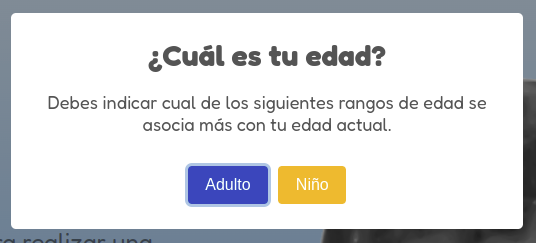
\includegraphics[width=0.4\textwidth]{imagenes/07_Implementacion/popup_edad.png}
        \label{fig:popup_edad}
    \end{subfigure}
    }
    \hfill
    \subfloat[Ventana emergente para la adquisición de permisos de envío de imágenes]{
    \begin{subfigure}
        \centering
        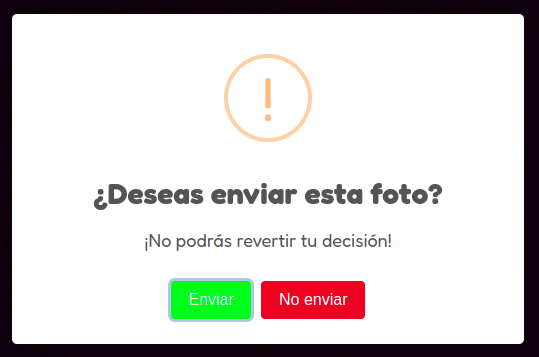
\includegraphics[width=0.5\textwidth]{imagenes/07_Implementacion/popup_enviar.png}
        \label{fig:popup_enviar}
    \end{subfigure}
    }
\caption{Ventanas emergentes de la Vista}
\end{figure}


\item \textbf{Permiso para el envío de la imagen tomada:} Esta ventana se lanza al pulsar sobre el botón de ``Enviar'' (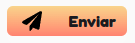
\includegraphics[width=0.15\textwidth]{imagenes/07_Implementacion/boton_enviar.png}) situado en la sección de captura de imágenes, el cual aparece una vez se ha capturado la imagen; y también se lanza cuando en el caso del móvil, se acepta enviar la imagen desde la aplicación de captura de imágenes del sistema. Esta última forma depende del dispositivo que se esté utilizando porque depende de la aplicación del sistema.

La ventana emergente informa al usuario de que se va a producir el envío de la imagen tomada por el dispositivo de captura, y, por lo tanto, si quiere o no que se realice el envío de la imagen en cuestión. Además, se indica que no se puede revertir la decisión, ya que al decidir no enviar la imagen se cierra la ventana emergente. Esta ventana se puede ver en la Figura \ref{fig:popup_enviar}.

En el caso de que el usuario confirme el envío de imágenes, se procederá a efectuar el envío de la imagen para su posterior análisis para deducir la edad del usuario. Durante el tiempo que dure el envío de la imagen y su análisis se mostrará una figura de carga para proporcionar feedback al usuario. En caso contrario, al negar el envío de la imagen por parte del usuario, se procederá a cerrar la ventana emergente y a esperar a que el usuario vuelva a tomar una imagen que le parezca adecuada y vuelva a iniciar el proceso de envío de la imagen.

\end{itemize}

\subsection{Interfaces web}

La interfaz web utilizada ha sido la proporcionada por las integraciones de Dialogflow. Ya que implementar una interfaz web propia llevaría cierto tiempo que está mejor invertido si se aprovecha en otras secciones del sistema, puesto que la interfaz que proporciona Dialogflow es adecuada para nuestro sistema. La posible ventaja que hemos perdido por no hacer nuestra propia interfaz es la pérdida de control en nuestro sistema, pues ahora hay un elemento que no podemos controlar su funcionamiento entorno y ni podemos modificarlo internamente.

Para obtener esta interfaz web debemos acceder al chatbot que hemos creado en Dialogflow. En nuestro caso hemos generado un agente por cada rango de edad. Lo hemos hecho de esta forma para diferenciar con que agente está charlando el usuario, ya que como hemos indicado anteriormente, al emplear una interfaz que no es nuestra, perdemos parte del control y en consecuencia, si tenemos un agente único, no podremos diferencia los mensajes de un usuario del rango de Adulto, de los mensajes de un usuario del rango de Niño.

Una vez nos encontramos dentro del agente en Dialogflow, nos dirigimos al apartado de Integrations, el cual se puede ver en la Figura \ref{fig:integrations_dialogflow}.

\begin{figure}[h]
\centering
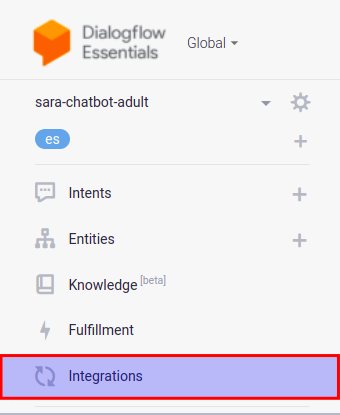
\includegraphics[width=0.4\textwidth]{imagenes/07_Implementacion/integrations_dialogflow.png}
\caption{Apartado Integrations de un agente de Dialogflow}
\label{fig:integrations_dialogflow}
\end{figure}

Dentro de este apartado nos dirigimos a la sección Text based donde se encuentra Web Demo, que es la interfaz web de Dialogflow. Este apartado se puede ver en su totatilidad en la Figura \ref{fig:text_based}.

\begin{figure}[h]
\centering
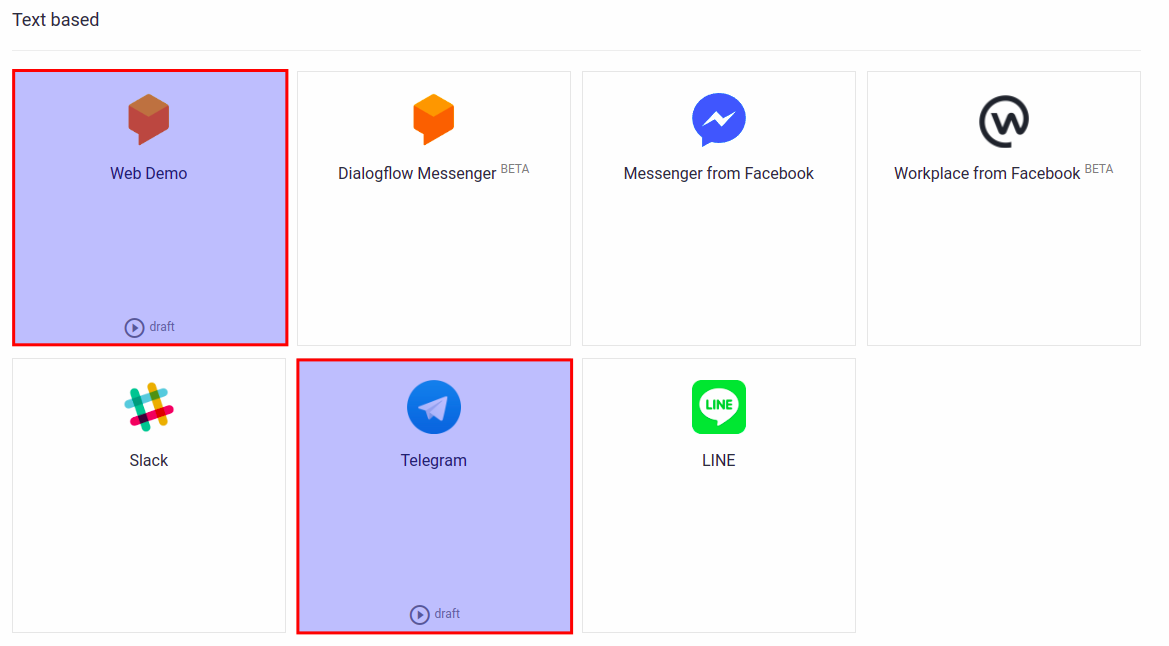
\includegraphics[width=0.6\textwidth]{imagenes/07_Implementacion/text_based.png}
\caption{Sección Text based del apartado Integrations}
\label{fig:text_based}
\end{figure}

Al pulsar sobre Web Demo aparece una ventana emergente donde se puede habilitar esta interfaz para el chatbot que se esté utilizando. Esta ventana emergente se puede ver en la Figura \ref{fig:web_demo}. Una vez habilitada se podrá hacer uso de ella mediante un iframe. Este iframe al colocarlo en un archivo HTML, incrustará el código HTML de la interfaz web de Dialogflow.

\begin{figure}[h]
\centering
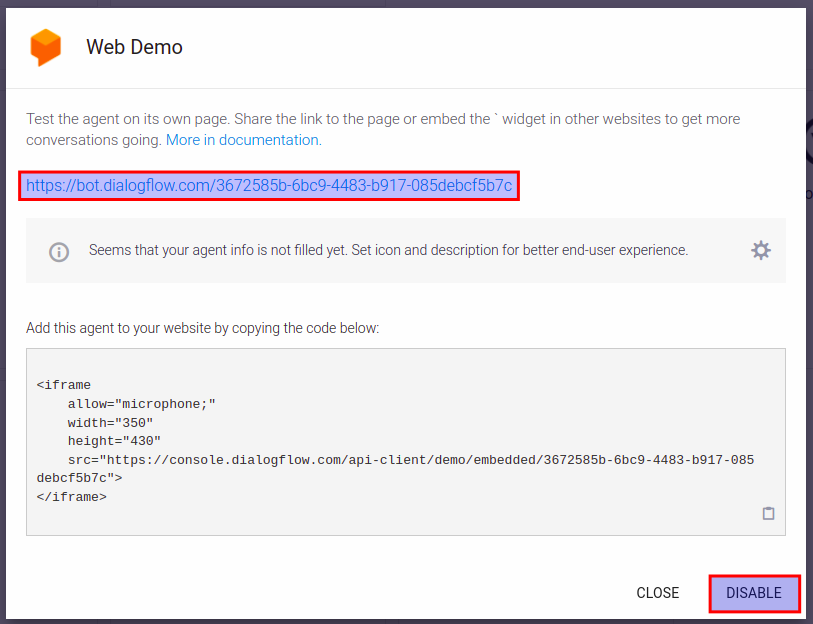
\includegraphics[width=0.7\textwidth]{imagenes/07_Implementacion/web_demo.png}
\caption{Ventana emergente de Web Demo de Dialogflow}
\label{fig:web_demo}
\end{figure}

Para obtener el código del iframe se accede a la URL que aparece marcada en la Figura \ref{fig:web_demo}. Al abrir esta URL nos abrirá una nueva ventana donde se puede ver el código del iframe del chatbot donde nos encontremos. Esta ventana se puede ver en la Figura \ref{fig:dialogflow_iframe}.

\begin{figure}[h]
\centering
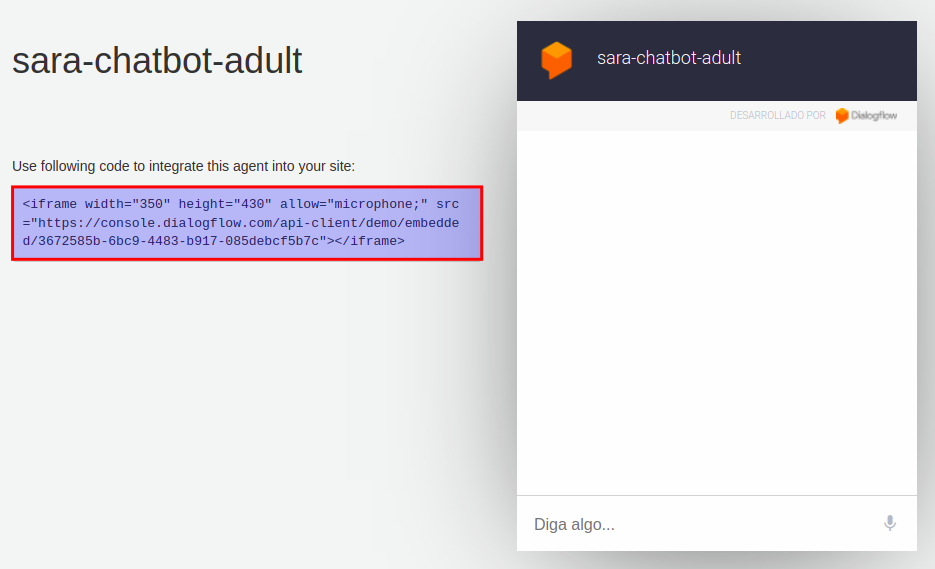
\includegraphics[width=0.7\textwidth]{imagenes/07_Implementacion/dialogflow_iframe.png}
\caption{Ventana donde se muestra el código del iframe}
\label{fig:dialogflow_iframe}
\end{figure}

El código del iframe de uno de los chatbots creados en Dialogflow se puede ver en la Figura \ref{fig:codigo_iframe}. Como se puede apreciar se indica el tamaño de ventana que tendrá la interfaz. Para que la interfaz se adapte al tamaño que nosotros le indiquemos en nuestro sitio web, se eliminan estos dos atributos del iframe. El siguiente atributo que aparece son los permisos que necesita la interfaz web. Como se puede ver se indica el micrófono, ya que además de poder introducir texto de forma escrita, también se puede introducir de forma oral; pero para ello es necesario que el usuario de permisos para el uso del micrófono por parte de nuestro sitio web. Y por último, el atributo que aparece al final es la dirección al código de la interfaz web, el cual será integrado en nuestro sitio web.

\begin{figure}[h]
\centering
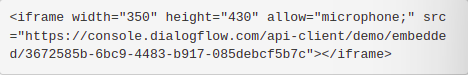
\includegraphics[width=0.7\textwidth]{imagenes/07_Implementacion/codigo_iframe.png}
\caption{Código del iframe del chatbot para adultos}
\label{fig:codigo_iframe}
\end{figure}

El aspecto final de nuestra interfaz web se puede ver en la Figura \ref{fig:interfaz_web}.

\begin{figure}[h]
\centering
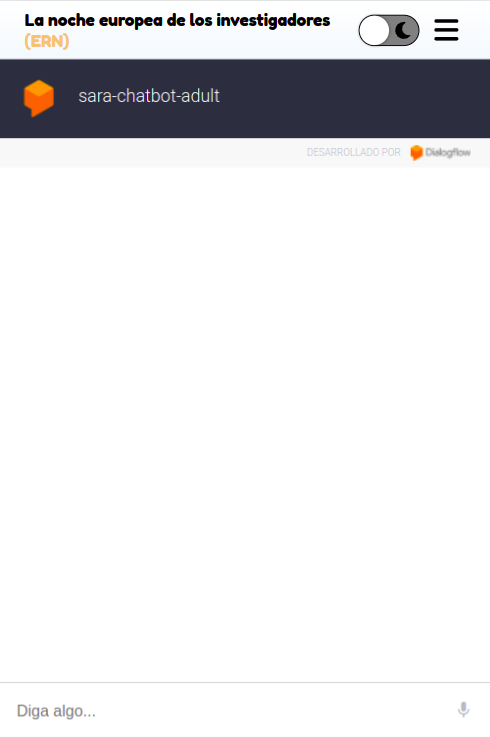
\includegraphics[width=0.4\textwidth]{imagenes/07_Implementacion/interfaz_web.png}
\caption{Aspecto de la interfaz web del chatbot para adultos desde una tablet en orientación vertical}
\label{fig:interfaz_web}
\end{figure}

\subsection{Interfaces de Telegram}

Para dar mayor acceso a nuestro chatbot se han elaborado interfaces para Telegram. De modo parecido a como se hace con la interfaz web, se ha hecho uso de las integraciones de Dialogflow, pero en este caso con Telegram. La sección de Telegram dentro del apartado de Integrations de Dialogflow se puede ver en la Figura \ref{fig:text_based}. Al pulsar en la sección de Telegram, aparecerá una ventana emergente parecida a la de Web Demo, donde se solicita el token del chatbot. Se solicita un token porque todos los bots en Telegram tienen asignado un token. Esta ventana emergente se puede ver en la Figura \ref{fig:token_telegram}.

\begin{figure}[h]
\centering
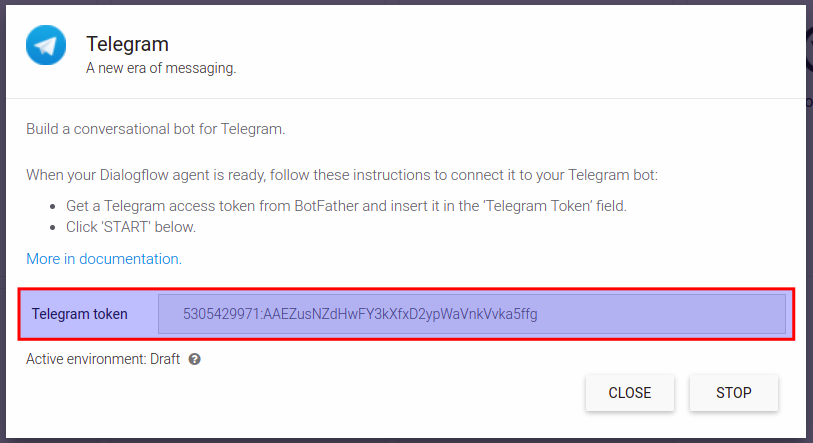
\includegraphics[width=0.6\textwidth]{imagenes/07_Implementacion/token_telegram.png}
\caption{Ventana emergente de Telegram de Dialogflow}
\label{fig:token_telegram}
\end{figure}

Por lo que llegados a este punto debemos crear un bot en la aplicación de Telegram, para poder hacer uso de él como interfaz para nuestro chatbot. Para generar un chatbot en Telegram se debe acceder a BotFather, que es un bot cuyo objetivo es la creación del resto de bots que existen en Telegram. El chat con este bot se puede ver en la Figura \ref{fig:bot_father}.

\begin{figure}[h]
\centering
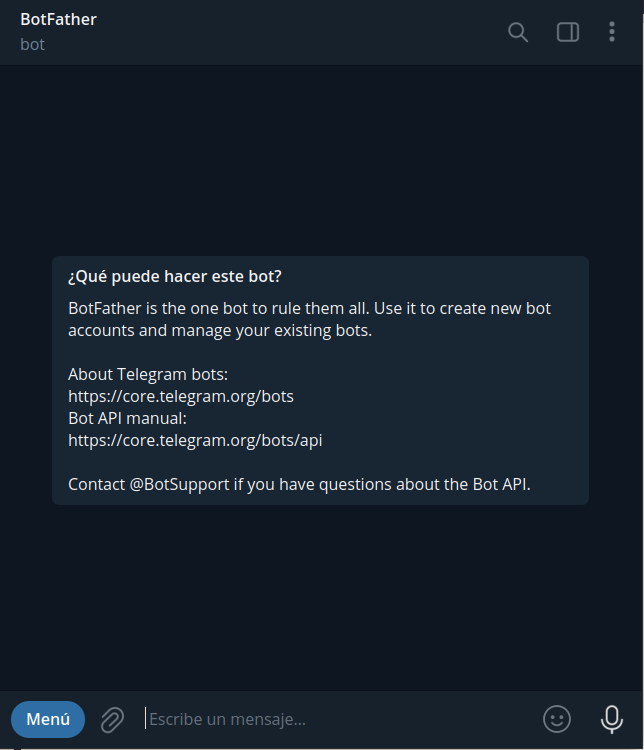
\includegraphics[width=0.4\textwidth]{imagenes/07_Implementacion/bot_father.png}
\caption{Chat con el bot de Telegram BotFather}
\label{fig:bot_father}
\end{figure}

Con el comando /newbot se inicia el proceso de creación del bot. Durante este proceso se nos solicita el nombre del bot; y posteriormente se nos solicita el username del bot, el cual debe terminar con la palabra "bot" o "Bot". Una vez terminado este proceso aparecerá un mensaje con el token asociado a nuestro nuevo bot. De la misma forma que para la interfaz web se producen dos chatbots en Dialogflow, para la interfaz de Telegram también se deben crear dos bots y obtener los tokens de ambos.

Una vez tenemos este token lo introducimos tal y como aparece en la Figura \ref{fig:token_telegram}.

El aspecto final de nuestra interfaz de Telegram será el que se muestra en la Figura \ref{fig:interfaz_telegram}.

\begin{figure}[h]
\centering
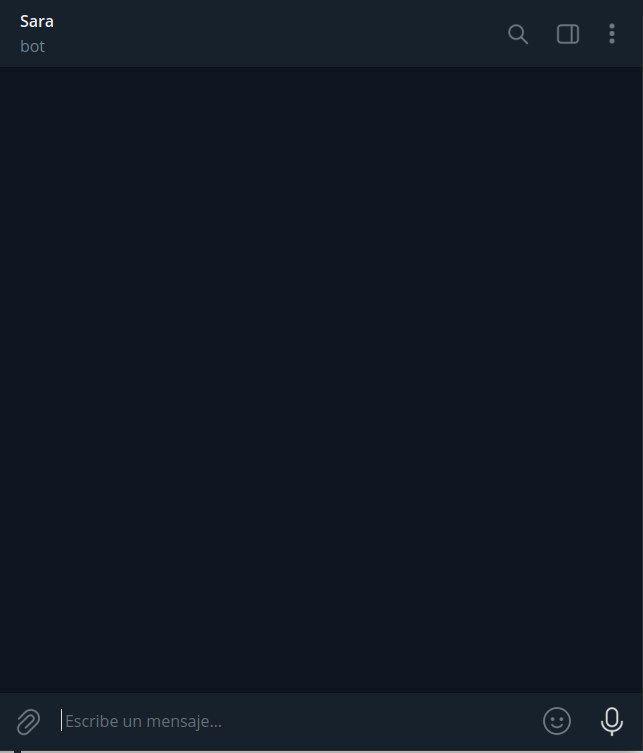
\includegraphics[width=0.4\textwidth]{imagenes/07_Implementacion/interfaz_telegram.png}
\caption{Aspecto de la interfaz de Telegram del chatbot para adultos}
\label{fig:interfaz_telegram}
\end{figure}


\section{Implementación del Controlador}

\subsection{Herramientas para el desarrollo} \label{subsec:herramientas_controlador}

Las herramientas usadas en el Controlador son muy diversas debido a la multitud de funcionalidades de este módulo, a su conexión con el resto de módulos y a su despliegue de forma pública.

En la implementación del Controlador se tendrá como lenguaje central al lenguaje de programación Python. La versión de Python utilizada será la versión 3.9.10.

Pero este lenguaje Python se utilizará en conjunto con otros lenguajes y herramientas dependiendo de la región del servidor que se esté implementando.

Para la parte de implementación de las conexiones con la Vista se empleará el lenguaje Javascript para elaborar las peticiones HTTPS que permiten la conexión con el Controlador. Y en pequeña medida se hará uso del lenguaje HTML5 para el paso de información útil.

Para el despliegue del servidor se hará empleo de un conjunto de herramientas como son Docker, Uvicorn, y de la plataforma Heroku \footnote{\url{https://heroku.com}}. Este despliegue se desarrollará más en detalle en el Apartado \ref{subsec:despl_servidor_heroku}.

Para la implementación de la estructura del servidor se hace empleo del lenguaje Python, aunque más en concreto se hace uso de un framework basado en Python como es FastAPI \footnote{\url{https://fastapi.tiangolo.com}}.

Para el resto de secciones, como puede ser la gestión de la conversación, se hará empleo únicamente del lenguaje Python.

\subsection{Implementación del servidor} \label{subsec:implementacion_controlador}

Dado que vamos a implementar el servidor con el lenguaje Python, disponemos de múltiples posibilidades para la implementación del mismo. Desde la implementación utilizando únicamente Python, hasta utilizar frameworks modernos basados en Python, como puede ser FastAPI.

En mi caso, he optado por la utilización del framework FastAPI, debido a que este tipo de framework te permite desarrollar API's rápidas y con un gran rendimiento sin demasiado poner demasiado esfuerzo en su desarrollo. Además, te dan un gran abanico de posibilidades para añadir de forma simple funcionalidades a nuestro servidor.

Por supuesto, existe una gran cantidad de frameworks basados en Python para la elaboración de API's, pero como se puede ver en la Figura \ref{fig:comparativa_fastapi}, donde se compara el rendimiento de distintos frameworks. El framework FastAPI es el que obtiene unos mejores resultados entre los frameworks basado en Python, de ahí su elección para nuestro servidor, ya que queremos que las peticiones al servidor se gestionen lo más rápido posible para agilizar la comunicación con el chatbot y el movimiento por el sitio web.

\begin{figure}[h]
\centering
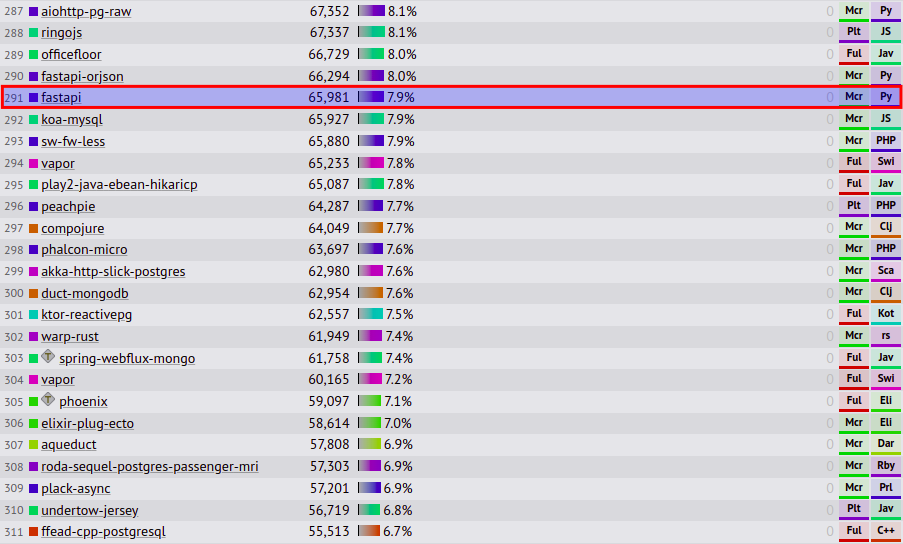
\includegraphics[width=0.8\textwidth]{imagenes/07_Implementacion/comparativa_fastapi.png}
\begin{center}
Fuente: \url{https://www.techempower.com/benchmarks/#section=data-r20&hw=ph&test=db}
\end{center}
\caption{Número de respuestas por segundo para peticiones (Datos del 02/08/2021)}
\label{fig:comparativa_fastapi}
\end{figure}

Una vez hemos elegido el framework con el que implementar el servidor, nos disponemos a explicar la forma en la que se realiza esta implementación con este framework en concreto. Muchos de los frameworks basados en Python siguen la metodología de FastAPI para la elaboración de servidores.

Lo primero que se debe hacer es la creación del servidor, para ello se hace uso de la función \textit{FastAPI}. Con esta función obtenemos un objeto con el que podremos definir las distintas secciones del servidor.

La definición de cada una de las secciones se componen de dos pasos. En primer lugar, se define el tipo de peticiones que recibe la sección, GET o POST; la ruta interna de la sección, la cual debe contener como mínimo la ruta raíz '/'; y por último el tipo de respuesta, que en el caso de nuestro servidor la respuesta puede ser código HTML o texto plano. En segundo punto, se define la función que se ejecutará al entrar a esa sección del servidor. Esta función deberá tener unos parámetros y unas salidas que estén en sintonía con el tipo de petición que se haya elegido en el primer paso.

Un ejemplo de definición de una sección del servidor se puede ver en la Figura \ref{fig:ejem_def_sec_servidor}.

\begin{figure}[h]
\centering
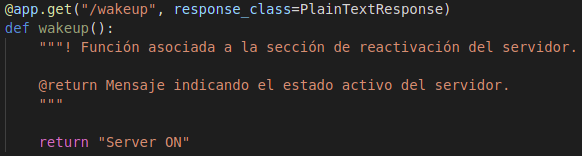
\includegraphics[width=0.7\textwidth]{imagenes/07_Implementacion/ejem_def_sec_servidor.png}
\caption{Ejemplo de definición de sección del servidor del Controlador}
\label{fig:ejem_def_sec_servidor}
\end{figure}

\subsection{Despliegue del servidor} \label{subsec:despl_servidor_heroku}

Como se ha indicado en la exposición de las herramientas del Controlador (Apartado \ref{subsec:herramientas_controlador}). Para el despliegue se hace uso principalmente de tres herramientas.

La primera herramienta a utilizar es Uvicorn. Uvicorn es un servidor ASGI basado en uvloop y httptools. Una hemos creado nuestro servidor con FastAPI, empleamos el mismo objeto con el que definíamos las secciones del servidor para ejecutar el servidor. Ayudándonos de la librería de Python de Uvicorn, utilizamos la función \textit{run} para ejecutar nuestro servidor FastAPI, pasándole como argumentos el objeto que define a la aplicación de FastAPI, el puerto en el que el servidor escuchará y la dirección de host. El puerto y la dirección host se pueden obtener tanto del archivo de configuración del servidor como de las variables de configuración de nuestra app en Heroku. Con esta información podremos ejecutar la aplicación de FastAPI mediante el módulo Uvicorn.

Pero hasta este punto únicamente tendríamos un servidor ejecutandose de forma local, situación que no es la conveniente para nuestro sistema, dado que sus objetivos es que pueda ser empleado por cualquier persona y en cualquier momento. Es por ello que en este punto entra en acción el uso de una plataforma como es Heroku. Y de la mano de Heroku viene la utilización de la herramienta Docker, de la que se hablará en los siguientes apartados.

Heroku es una plataforma de tipo PaaS que permite a los desarrolladores implementar, ejecutar y trabajar con aplicaciones que se estén ejecutando en su totalidad en la nube. De esta manera, al ejecutar nuestro servidor en esta plataforma, dispondremos de un punto de acceso público a nuestro sitio web y a todas las funcionalidades que proporciona.

Una vez sabemos de qué se trata la plataforma Heroku, debemos concretar como se traspasa nuestro trabajo realizado de forma local en nuestra máquina a un espacio de trabajo en la nube.

Este despliegue a la plataforma Heroku se puede efectuar por tres vías. Una vez que creamos nuestra app en la plataforma de Heroku, si accedemos a la misma y nos vamos a la sección Deploy, podremos ver las tres vías que existen. Estas vías se pueden ver en la Figura \ref{fig:deploy_heroku}.

\begin{figure}[h]
\centering
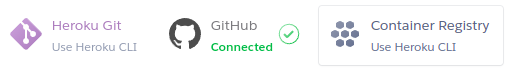
\includegraphics[width=0.7\textwidth]{imagenes/07_Implementacion/deploy_heroku.png}
\caption{Métodos de despliegue de apps en Heroku}
\label{fig:deploy_heroku}
\end{figure}

En mi caso he optado por el tercer método, el cual involucra a los contenedores. Por esta razón se menciona en anteriores párrafos el uso de Docker, ya que se efectuará el despliegue de la app como un contenedor. Las ventajas de los contenedores son que producen una menor sobrecarga, permiten una mayor portabilidad, y son más eficientes, entre muchos otros.

Los pasos a seguir siguiendo este método se explican en el apartado Container Registry \footnote{\url{https://dashboard.heroku.com/apps/sara-chatbot-tfg/deploy/heroku-container}} de la sección Deploy de la app. Los únicos requisitos para este método es tener instalado en el sistema tanto Heroku CLI como Docker.

Pero yo he seguido una vía alternativa, dado que estamos usando Github como plataforma para el control del código del proyecto, he optado por sacar potencial a la funcionalidad de los Workflows que se nos proporciona en Github. Estos Workflows no son más que procesos automatizados que se pueden configurar con uno o más trabajos. Para la creación de los archivos que componen a estos Workflows se hace empleo del lenguaje YAML.

Basándonos en estos Workflow he configurado un trabajo que realiza el despliegue del Controlador en la plataforma Heroku de forma automática cuando se percibe por parte de Github que ha habido cambios en el código del Controlador.

Además, para una mayor capacidad de configuración se ha hecho uso de los Actions secrets de Github. Esta funcionalidad de Github permite guardar valores en variables que puede ser utilizadas desde los trabajos de los Workflows, y siendo además privados, por lo que se pueden guardar datos sensibles como contraseñas.

Siguiendo con el trabajo que efectúa el despliegue del Controlador, este trabajo se podría haber implementado en su totalidad por mí, pero para ahorrar tiempo y evitar errores que pudiesen surgir he optado por usar un Action creado por otra persona. Los trabajos de los Workflows se componen de una serie de Actions. El Action utilizado pertenece a AkhileshNS y se llama \href{https://github.com/AkhileshNS/heroku-deploy}{heroku-deploy}. Para facilitar el uso de este Action se dispone de ejemplos de uso en su repositorio de Github. Los datos que requiere este Action para realizar el despliegue es la API key de nuestra cuenta de Heroku, el nombre que le hemos asignado a nuestra app a la hora de generarla en Heroku, en nuestro caso es sara-chatbot-tfg, el email empleado a la hora de registrarnos en la plataforma de Heroku, y por último el directorio donde se encuentra el Dockerfile que define al contenedor. Los tres primeros datos estarán guardados en tres variables distintas dentro de los Actions secrets de nuestro repositorio de GitHub, donde se controla el código de nuestro proyecto.

Hasta este punto tenemos una forma de efectuar el despliegue automático, pero necesitamos definir como debe formarse el contenedor. Como se ha indicado en el anterior párrafo, al Action es necesario indicarle donde se encuentra un archivo en concreto, el Dockerfile. Este archivo es vital para la elaboración de un contenedor. Un Dockerfile es un archivo de texto simple que define un conjunto de comandos que se ejecutará para formar el entorno del contenedor. Para generar nuestro contenedor del Controlador hemos usado como base del contenedor una imagen de Python cuya versión es 3.9.10\ . Posteriormente, se copia todo el contenido del directorio, incluido el propio directorio, que contiene todo el código del Controlador en la raíz del contenedor. Después de realizar la copia se establece como directorio de trabajo el propio directorio que se ha copia en el contenedor. Seguidamente, procedemos a la instalación de los requisitos del Controlador mediante el comando pip. Y finalmente, establecemos como punto de entrada al contenedor la ejecución del script main.py, el cual ejecutará el inicio del servidor del Controlador.

Después de todos lo dicho ya tendríamos un servidor para el Controlador al que se puede acceder de forma pública y en cualquier momento.

Aunque el trabajo que efectúa el despliegue no es el único que he elaborado relacionado con el Controlador, ya que puesto que estamos usando contenedores para realizar el despliegue, pensé que era buena idea subir el contenedor que se obtiene con el controlador a la plataforma DockerHub \footnote{\url{https://hub.docker.com}}. Esta plataforma es el equivalente a GitHub para contenedores, sirve como plataforma para albergar contenedores en repositorios privados o públicos. Esta subida se hace con otro trabajo dentro del mismo Workflow del despliegue del Controlador para aprovechar la automatización lograda. El único requisito para proceder a la subida es tener instalado en la máquina el paquete Docker. Una vez lo tenemos instalado la subida consiste en los siguientes pasos:

\begin{itemize}
\item Login en la plataforma de DockerHub con nuestro usuario y contraseña
\item Construcción de la imagen del contenedor
\item Subida de la imagen al repositorio \href{https://hub.docker.com/repository/docker/macarse/sara-chatbot-controller}{sara-chatbot-controller}
\end{itemize}

Ahora, al disponer de la imagen del contenedor en un repositorio, se podría cambiar fácilmente la plataforma donde se despliega siempre y cuando se pueda efectuar el despliegue mediante contenedores.

Llegados a este punto tendríamos una estructura de despliegue del Controlador totalmente automatizada.


\subsection{Gestión del sitio web} \label{subsec:gest_sitio_web}

Una de las ventajas de usar FastAPI para la implementación del servidor es la posibilidad de utilizar cualquier motor para las plantillas HTML. Para el caso de nuestro servidor he optado por Jinja2, que es el motor que se recomienda en la documentación de FastAPI y el cual es frecuentemente empleado en otros frameworks. El único requisito para el uso de este gestor de plantillas es la instalación de la librería de Python \textit{jinja2}.

Para un fácil empleo de este gestor aparecen ejemplos de uso del mismo en la documentación de FastAPI \footnote{\url{https://fastapi.tiangolo.com/advanced/templates}}.

Para hacer uso del gestor en nuestro servidor es necesario seguir los siguientes pasos:

\begin{itemize}
\item Importar Jinja2Template de la librería fastapi.templating\ .
\item Montaje de los archivos de la carpeta static, carpeta cuyo contenido es todo aquel distinto de las plantillas HTML.
\item Creación del objeto templates con el cual se podrán manejar las plantillas
\item Declaración de un parámetro de tipo Request en cada una de las funciones asociadas a una ruta que devuelve una plantilla HTML. Además, cada una de estas funciones debe devolver una plantilla.
\item Generación de una plantilla renderizada mediante el objeto templates obtenido en el tercer paso.
\end{itemize}

Para generar una plantilla renderizada se hace del método TemplateResponse del objeto templates. Este método requiere de dos parámetros. El primer parámetro será una cadena con la ruta relativa de la plantilla que se quiere renderizar. Esta ruta relativa tomará como base el directorio que se indicó en la creación del objeto templates, este directorio es el directorio que contiene todas las plantillas del servidor llamado templates. El segundo parámetro será un diccionario donde cada par clave-valor estará compuesto por una cadena que será la clave y por una variable que será el valor. Es importante la cadena que se utilice como clave, ya que con ese nombre se podrá acceder al valor asignado desde el código de las plantillas. Algo relevante a destacar es que al menos este diccionario debe tener un elemento, el cual es el parámetro de tipo Request que se indicó en la lista de pasos.

Con lo comentado hasta este momento podríamos tener un servidor web totalmente funcional en cuanto a lo estético, pero para poder realizar algunas de las funcionalidades del sitio web es necesario hacer uso de las posibilidades que nos da el gestor Jinja2 con el paso de valores a través del diccionario que se comentó anteriormente. A través de este diccionario se pasará la información que requieran las plantillas y el cual no se pueda saber de forma estática, sino dinámica. Algunos ejemplos de este tipo de información pueden ser el estado del modo oscuro, es decir, si está activado o no; o la URL del servidor GPU, la cual puede cambiar durante la ejecución del Controlador si se inicia varias veces el servidor del Modelo durante la ejecución del servidor del Controlador.

Pero haciendo empleo del diccionario hacemos que esta información únicamente sea accesible desde la plantilla, pero no desde el código Javascript, que es donde realmente es necesaria esta información, ya que es el lugar donde se ejecuta la lógica de las plantillas. Para acceder a la información de una clave se debe escribir en la plantilla de código HTML el nombre de la clave dentro de dos llaves a ambos lados, es decir, si la clave se llama estado para acceder a su valor se debe escribir \{\{estado\}\}. Esta forma de acceder a la información solamente es posible desde el código HTML, en este punto es donde entra en juego el uso del lenguaje HTML dentro de la implementación del Controlador, la cual se mencionó en el apartado de herramientas de desarrollo del Controlador (Apartado \ref{subsec:herramientas_controlador}).

Para poder acceder a esta información desde los scripts de Javascript se creará un párrafo de HTML para cada clave que se pase al diccionario, el cual contendrá la información de esa clave. Este párrafo tendrá un estilo que le otorgue la visibilidad de oculto. Y para acceder a la información se obtendrá el elemento HTML desde el script de Javascript y ya tendremos acceso a esa información. Un ejemplo de definición de un párrafo para una clave se puede ver en la Figura \ref{fig:def_clave_jinja}.

\begin{figure}[h]
\centering
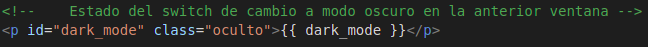
\includegraphics[width=0.8\textwidth]{imagenes/07_Implementacion/def_clave_jinja.png}
\caption{Ejemplo de definición de una clave en una plantilla HTML}
\label{fig:def_clave_jinja}
\end{figure}

\subsection{Secciones adicionales del servidor}

En este apartado se abordan las secciones del servidor del Controlador que no están orientadas al sitio web, sino que han surgido como solución a algún problema que haya surgido durante el desarrollo del servidor. En concreto, estamos hablando de dos secciones. Por un lado, una sección para la reactivación del servidor cada cierto tiempo; y, por otro lado, una sección para la actualización de la URL pública del servidor del Modelo.

\subsubsection*{Sección para la reactivación del servidor}

Por supuesto, la versión gratuita de Heroku tiene sus inconvenientes, principalmente enfocados en la actividad del servidor. El primer inconveniente se trata de una limitación en el uso de los recursos que nos proporciona la plataforma. Como se indicó en el apartado de gestión del proyecto, la plataforma Heroku dispone de unas unidades llamadas dynos, que son las encargadas de ejecutar nuestras apps. Con la versión gratuita, que es la que estamos utilizando, disponemos de una cuota de 550 horas gratuitas de utilización de los dynos. Esta cuota se renueva mensualmente. Esta información se puede comprobar en la sección de la documentación de Heroku sobre el empleo de los dynos gratuitos \footnote{\url{https://devcenter.heroku.com/articles/free-dyno-hours#usage}}. Además, esas 550 horas son horas de utilización con un único dyno, en el caso de usar dos dynos para nuestra app, dispondríamos de 275 horas gratuitas en total, es decir, la mitad. Si comparamos esta cantidad de horas, 550 horas, con la cantidad de horas de las que dispone como máximo un mes, las cuales son 744 horas, vemos como el número de horas que nos proporciona la versión gratuita se queda corta para poder proporcionar un servicio continuo del servidor. En el caso de que nuestra app supere la cuota de uso de nuestra cuenta, todos los dynos que estén ejecutando nuestras apps entrarán de forma forzosa en estado inactivo, dejando sin servicio a todas nuestras hasta que se vuelve a renovar la cuota de uso.

Para poder superar esta diferencia de horas sin tener llegar al apagado forzoso de los dynos, debemos hallar una solución para aumentar nuestra cuota de uso hasta llegar a una cuota que nos permita dar un servicio continuo. La plataforma Heroku nos da la posibilidad de aumentar esta cantidad de horas simplemente introduciendo los datos de la tarjeta de crédito en nuestra cuenta, sin tener que realizar ningún pago. La plataforma nos dará 1000 horas por el simple hecho de introducir estos datos. De esta manera superamos las 744 horas que puede tener como máximo un mes del año.

Un tip que es interesante para llevar el control del consumo de nuestra cuota de utilización de los dynos es hacer uso de Heroku CLI mediante el comando \textit{heroku ps -a name&gt;}, con el cual obtendremos el porcentaje de la cuota que ya ha sido usado y el número de horas restante de la cuota. Aunque alternativamente se puede controlar este consumo de la cuota desde el apartado de pagos de nuestra cuenta, por si el administrador del sistema le es más agradable tener una interfaz gráfica para realizar este control.

Pero si analizamos el primer inconveniente, vemos como no tiene influencia en la implementación del servidor, y así es, aunque este no es el único inconveniente derivado del uso de la cuenta gratuita. El otro inconveniente de este tipo de cuenta es que los dynos que están ejecutando nuestro sitio web entran en estado inactivo al trascurrir cierto tiempo sin actividad en el servidor, de esta forma la plataforma no está gastando recursos de forma innecesaria. Esta desconexión de los dynos al no detectar actividad en la app se explican en la sección de la documentación de Heroku sobre la inactividad de los dynos \footnote{\url{https://devcenter.heroku.com/articles/free-dyno-hours#dyno-sleeping}}. Este paso a estado inactivo es un problema, ya que cuando se vuelve a tener actividad en el servidor se deberá volver a iniciar el servidor, lo que conllevará una espera que no será agradable para el usuario. A diferencia del primer inconveniente, Heroku no nos proporciona una solución a este segundo inconveniente, por lo que habrá que buscar una solución provisional para este inconveniente. Una solución provisional que se suele usar es la ejecución de comandos ping al servidor de manera periódica. Para la ejecución periódica de estos comandos se hace empleo de la plataforma \href{https://console.cron-job.org/}{cron-job}. Dentro de esta plataforma se pueden crear trabajos que se ejecutan cada cierto tiempo, tiempo que se puede definir en el trabajo. Estos trabajos ejecutan un comando ping a la dirección URL que se le indique en el trabajo. Para gestionar estos ping al servidor se ha generado la sección wakeup en el servidor del Controlador. A esta sección será a la que se realicen los comandos ping. Esta sección lo único que hace es devolver un texto plano indicando el estado activo del servidor.

Después de aplicar estas dos soluciones tendremos un servidor disponible en cualquier momento.

\subsubsection*{Sección para la actualización de la URL pública del servidor del Modelo}

La gestión de la actualización de la URL pública del servidor es de igual forma importante para asegurar un servicio continuo del sitio web. Ya que puede darse el caso de que el servidor del Modelo se reinicie por cualquier motivo y cambie la URL pública del servidor. Esto sucede porque la URL pública del servidor se genera nuevamente cada vez que se inicia el servidor y cada vez que se genera es distinta. Esto sucede por la forma en que se ha implementado, lo cual se explicará en la sección de implementación del Modelo (Apartado \ref{sec:implementacion_modelo}).

Para gestionar este cambio dinámico de la URL, se ha creado una sección en el servidor del Controlador, donde se actualiza la variable que contiene la URL pública del servidor del Modelo. Esta sección se llama \textit{setURL}. Esta sección recibirá peticiones POST del servidor del Modelo, cuando se necesite actualizar la URL. Se necesitará actualizar la URL en los siguientes casos:

\begin{itemize}
\item Inicio del servidor del Modelo
\item Reinicio del servidor del Modelo
\item Inicio o reinicio del servidor del Controlador cuando el servidor del Modelo ya está activo.
\end{itemize}

Con el último caso descrito se deberá ejecutar una sección del servidor del Modelo para realizar la actualización. Este proceso se describirá en la sección de implementación del Modelo (Apartado \ref{sec:implementacion_modelo}).

La lógica de la sección generada es simple. Únicamente se recibe una petición POST que contiene la URL pública del servidor del Modelo, se extrae esa URL de la petición y finalmente se asigna el valor de la URL a la variable que contendrá el valor de la misma para poder ser usado por el resto de secciones del servidor.


\subsection{Procesado de las imágenes}

El procesado de las imágenes se realiza de forma distinta dependiendo del dispositivo que se esté utilizando. Aunque todo el procesado de las imágenes realizado por el Controlador se ha implementado en scripts de Javascript.

Si se usa un móvil, esta sección únicamente se compone de una parte, dado que el mismo botón de captura de la imagen lanza el envío de la imagen. Al pulsar sobre el botón de captura se lanzará la aplicación del sistema, la cual se encarga de capturar una imagen y preguntar al usuario si quiere utilizar esa imagen para la deducción de la edad. Una vez hemos aceptado cuál será nuestra imagen, el usuario será preguntado por el sistema por el permiso para el envío de la imagen. Si el usuario acepta el envío, se procederá a realizar el mismo. El envío consistirá en la lectura de la imagen en formato base64, seguido del envío de la imagen dentro de una petición POST a la ruta de deducción de edad del servidor del Modelo. Como respuesta a esta petición obtendremos el rango de edad que se ha deducido. Dependiendo de este rango de edad se abrirá una interfaz u otras, pero también habrá que tener en cuenta el canal que ha elegido el usuario. El canal elegido, la URL del servidor del Modelo, y la dirección a cada una de las interfaces disponibles se pasará al script a través del paso de valores con el módulo Jinja2, tal y como se indica en el Apartado \ref{subsec:gest_sitio_web}.

En el caso de usar otro dispositivo distinto del móvil, esta sección estará compuesta de dos partes. En la primera parte se realiza el mismo proceso que se realiza en la aplicación del sistema en el caso del móvil, aunque en este caso en vez de ver la imagen en la aplicación de captura de imágenes del sistema, se verá un elemento que mostrará el vídeo captado por la cámara del dispositivo y otro elemento que será un canvas que almacenará la imagen que se captura del vídeo mencionado, ya que un vídeo no deja de ser una visualización continua de muchas imágenes. Una vez hemos captura la imagen y la tenemos en el canvas, tendremos un botón para iniciar el envío de la imagen. Este botón lanza la misma ventana en el otro caso para pedir el permiso de envío de la imagen. El envío de la imagen se efectúa de forma similar a como se hace en el otro caso, cambiado únicamente la forma en que obtiene la imagen, ya que en vez de leer la imagen de un archivo, se debe extraer la imagen almacenada en el canvas y pasarla a formato base64. La información externa que se necesita para realizar el envío se obtiene de igual forma con el paso de valores con el módulo Jinja2.

\subsection{Gestión de la conversación}

La manera de gestionar la conversación por parte del Controlador está muy condicionada por el uso de las interfaces que proporciona Dialogflow. Dado que, como se ha mencionado en la implementación de la Vista, todo lo que sucede dentro de la interfaz no se puede controlar, ni siquiera los mensajes. Por ello se debe hacer uso de una funcionalidad que tiene Dialogflow, que es el Webhook. En esta sección de Dialogflow se deberá introducir una URL que servirá como punto de conexión entre Dialogflow y el servidor que funcione como webhook del chatbot. La URL que se colocará será aquella que nos lleve a la sección de webhook del servidor del Controlador. Habrá una sección de webhook por cada rango de edad, ya que habrá que gestionar por separado las interfaces de adulto y de niño. En cada uno de los Intents del chatbot de Dialogflow se activará la llamada al webhook, de esta forma cuando se active uno de los Intent se realizará el envío de una petición POST al webhook. Esta petición contendrá información de la conversación, como puede ser el Intent que se ha activado, el texto de entrada que ha activado al Intent o el contexto del chatbot.

La gestión de la petición de Dialogflow por parte del Controlador se efectúa de manera similar independientemente del rango de edad, el único cambio es que la respuesta se obtiene efectuando la llamada a secciones distintas del servidor del Modelo. La gestión de la petición comienza obteniendo el Intent que lanzó la petición, ya que según el Intent se realizan algunos pasos distintos. El chatbot tendrá dos Intents, el Intent Talk y el Intent Goodbye. En el Intent Talk se efectúa toda la conversación, excepto la última interacción con el chatbot, que se realiza en el Intent Goodbye.

Si se trata del Intent Talk, el siguiente paso será comprobar si se trata de la primera generación de respuesta o no. Para obtener esta información se revisa el contexto que contiene la petición. Si dentro del contexto está el campo edad quiere decir que no es la primera respuesta, en caso contrario indica que si se trata de la primera respuesta.

Cuando se trata de la primera generación de respuesta, primeramente se verifica si el servidor del Modelo se encuentra activo. Si no se encuentra activo se le indica al usuario mediante una respuesta a través del chatbot. Si se encuentra activo, se extrae la información necesaria del contexto de la petición para efectuar la generación de la respuesta. Esta información es el texto de entrada y la edad, la cual se deduce de forma sencilla al ver a que webhook ha llegado la petición. Una vez se ha generado la respuesta, se elaborará el primer contexto de la conversación. Para la elaboración de este primer contexto será necesario obtener la fecha actual, que marcará el inicio de la conversación. Al contexto se añadirá la información de la fecha de inicio, la edad del usuario, se incluirá la entrada y la salida que se ha generado a partir de esa entrada y finalmente se añadirá el identificador de la conversación, el cual es muy importante para seguir la conversación en el resto de llamadas al webhook. La respuesta a la petición del webhook estará compuesta por el texto que se ha generado como respuesta al texto de entrada, y por el nuevo contexto que se ha generado.

Cuando se trata del resto de generaciones de respuestas, habrá pasos que se eviten sustituyéndolos por otros. En este caso, a la hora de generar la respuesta será necesario, el texto de entrada, al igual que pasaba en el otro caso; la edad, que en este caso se extraerá del contexto de la petición; y el identificador de la conversación, para indicar al Modelo de que se trata de una respuesta que continúa una conversación ya empezada. La generación del contexto evitará el añadir la fecha de inicio y la edad, ya que fueron añadidos en la primera generación. En esta generación de contexto solamente se añadirá el texto de entrada y la respuesta a la misma, y se actualizará el identificador de la conversación. La respuesta a la petición del webhook se elaborará de la misma forma.

Una vez hemos detallado el proceso con el Intent Talk. Si se trata del Intent Goodbye, los pasos a seguir son exactamente iguales a los realizados con el Intent Talk cuando no es la primera generación, con la única salvedad de que al final de todos los pasos se guardará la conversación en el log del sistema, para poder utilizar esta información para futuras mejoras del chatbot y también para el análisis de las conversaciones que se han realizado con el chatbot. El contexto no se guarda tal cual en el log, sino que más bien se formatea la información del contexto para guardarla de una manera clara en ella. Cabe destacar que antes de guardar la conversación se debe obtener la fecha actual para usarla como la fecha de finalización de la conversación. El guardado de la conversación en el log se explica en el Apartado \ref{subsec:guardado_conver}.

La generación de la respuesta consistirá en el envío de una petición al servidor del Modelo. La petición se enviará a la sección del servidor del Modelo acorde con la edad que se haya indicado a la función de generación de respuestas. Esta petición contendrá como información el texto de entrada, el identificador de la conversación en caso de conocerse, y un indicador de si es la última respuesta, información que es útil para el Modelo para su propia gestión de las conversaciones. La respuesta se obtendrá de la respuesta a esta petición al servidor del Modelo.

El contexto que se encuentra dentro de la petición al webhook está compuesto de varios elementos, ya que un chatbot en Dialogflow puede tener un contexto compuesto de varios elementos, donde cada elemento tenga cierta información. Pero para nuestro chatbot toda la información se guardará en el mismo elemento. El contexto donde se guardará toda la información será el llamado \textit{talk-followup}.

\subsection{Guardado de la conversación en el log} \label{subsec:guardado_conver}

Para facilitar la implementación del log de nuestro sistema, se ha hecho uso de las múltiples funcionalidades que proporciona Heroku a través de sus Add-ons. En concreto existe el Add-ons llamado Heroku Postgres, el cual crea una base de datos Postgres que es accesible desde la app de Heroku, y que hará la función de log del sistema. Este Add-ons se puede añadir de forma gratuita a nuestra app. Al instalar este Add-ons se añade de manera automática la URL del log a las variables de configuración de nuestra app. Este último punto es importante, ya que será necesaria esta URL para realizar las conexiones con el log desde nuestro código del servidor del Controlador.

Para efectuar la conexión se sigue la documentación de Heroku relaciona con la conexión del log con Python \footnote{\href{https://devcenter.heroku.com/articles/connecting-heroku-postgres#connecting-in-python}{https://devcenter.heroku.com/articles/connecting-heroku-postgres}}. En primer lugar, será necesario tener instalada la librería \textit{psycopg2-binary}. Dentro del código del servidor se hará import de la librería para poder acceder al log de la app. El primer paso para acceder al log, es la conexión con la misma. La conexión se realiza mediante la función connect de la librería. Esta función requiere de la URL del log, la cual se puede obtener mediante las variables de configuración de nuestra app. Esta función devolverá un objeto que representará la conexión con el log. Una vez hemos efectuado la conexión, debemos ver como escribir los datos de la conversación en el log, para ello es necesario obtener el cursor del log. Con este cursor se podrán ejecutar comando SQL sobre el log utilizando los datos de la conversación. Antes de realizar la escritura de los datos se deberán obtener las conversaciones con un formato claro, para facilitar su análisis en el log. Finalmente, cuando tenemos todos los datos listos, ejecutamos un comando INSERT sobre la tabla que contendrá las conversaciones. Este comando insertará la edad del usuario, la fecha de inicio de la conversación, la fecha de finalización de la misma y el contenido de la conversación, es decir, las distintas entradas y salidas de la conversación.

Cuando ya hemos insertado los datos en la tabla debemos comunicar al log los cambios mediante la función \textit{commit}. De esta forma, los cambios se harán permanentes en el log. Llegados a este punto ya hemos terminado el guardado de la conversación, por lo tanto, ya podemos cerrar tanto el cursor como el log. Ambos cierres se realizan con la función \textit{close} aunque sobre distintos objetos.


\section{Implementación del Modelo} \label{sec:implementacion_modelo}

\subsection{Herramientas para el desarrollo}

Las herramientas usadas en el Modelo, al igual que pasa en el Controlador, son muy diversas. Aunque hay ciertas herramientas que coinciden en ambas partes del sistema.

Toda la implementación del Modelo se realizará con el lenguaje de programación Python. La versión de Python utilizada será la versión 3.9.10\ .

Las herramientas comunes se encuentran en la sección de implementación y despliegue del servidor del Modelo. En cuanto a la implementación de la estructura del servidor, se hace empleo del framework FastAPI. Para el despliegue, a diferencia de lo que pasa con el Controlador, se deja de utilizar la herramienta Docker. Aunque se podría usar la herramienta Docker en caso de que fuese útil para una mejora de la calidad del sistema. La herramienta que si se emplea para el despliegue del servidor es la herramienta Uvicorn. Otra herramienta que no se emplea para el despliegue es la plataforma Heroku. No se hace uso de esta plataforma por la simple razón de que no dispone de apps con servicio de GPU. Por ello, para realizar el despliegue del servidor del Modelo se ha empleado la herramienta Ngrok, para realizar el despliegue de forma local en el servidor GPU del Instituto DaSCI y poder generar un punto de acceso público al servidor del Modelo.

Una parte fundamental del Modelo es la generación de respuestas, ya que es básica para la elaboración del chatbot. Como se ha comentado en el diseño del Modelo, esta generación de respuestas se va a basar en modelo pre entrenados del chatbot BlenderBot. Es en este punto cuando interviene el uso de la plataforma Huggingface \footnote{\url{https://huggingface.co/}}. Esta plataforma sirve como una base de modelos que son subidos por la comunidad. El modelo pre entrenado utilizado para toda la generación de respuestas es el modelo \href{https://huggingface.co/facebook/blenderbot-400M-distill}{blenderbot-400M-distill} de la empresa Facebook.

Si nos fijamos en el lenguaje empleado por el modelo de generación de respuestas, vemos que trabaja con texto en inglés, por lo tanto, será necesario traducir el texto de español a inglés y viceversa. Para nuestro sistema hemos empleado la API de DeepL, la cual nos permite tener un traductor varias veces mejor que el resto de traductores disponibles actualmente.

Otra sección del Modelo que ha hecho uso de la plataforma Huggingface, es la deducción de la edad a través de imágenes. Para reducir el tiempo de desarrollo del sistema sin dejar tener un sistema fiable, he optado por usar un modelo pre entrenado de clasificación de imágenes, el cual es capaz de clasificar una imagen de una persona en un rango de edad concreto. El modelo utilizado es \href{https://huggingface.co/nateraw/vit-age-classifier}{vit-age-classifier} del desarrollador nateraw.

\subsection{Implementación del servidor}

Dado que en la sección de herramientas se ha indicado que la implementación de la estructura del servidor se realizaría con el framework FastAPI, la implementación llevada a cabo para el servidor del Modelo no diferirá mucho de la implementación del servidor del Controlador, la cual se puede ver en el Apartado \ref{subsec:implementacion_controlador}. Una de las diferencias será el número y la funcionalidad de las secciones del servidor, y la otra diferencia estará relacionada con el intercambio de información entre los servidores. Esta última diferencia viene originada por la propia estructura de nuestro sistema, ya que debemos implementar dos servidores con dominio distinto que se comunican entre ellos. Este intercambio de información tiene especial importancia en las comunicaciones entre la interfaz y el servidor del Modelo. Dado que la interfaz del sistema se encuentra en el dominio del servidor del Controlador y el servidor del Modelo se encuentra en un dominio distinto, deberemos añadir ciertas cabeceras en las conexiones entre ambas partes del sistema.

Estas cabeceras con las llamadas cabeceras CORS o cabeceras de Intercambio de recursos de origen cruzado. Dado que para la implementación del servidor se hace uso del framework FastAPI, utilizaremos las herramientas que nos proporciona este framework para solucionar este problema. La herramienta a utilizar en este caso es la adhesión de un middleware de tipo CORS, para ello se debe hacer uso de la función \textit{add\_middleware} y de la clase \textit{CORSMiddleware}. Como se indica en \href{https://fastapi.tiangolo.com/tutorial/cors/}{la documentación de FastAPI}, este tipo de middleware se utiliza en situaciones en las que la interfaz tiene código Javascript que se comunica con un backend y el backend está en un dominio diferente al de la interfaz.

\subsection{Despliegue del servidor}

Para el despliegue del servidor se hace uso de dos herramientas, una de ellas ya empleada para el despliegue del servidor del Controlador.

La herramienta que ya ha sido utilizada es Uvicorn. Esta herramienta, como ya se explicó en el despliegue del Controlador, es un servidor ASGI el cual nos permite poner en funcionamiento la estructura de nuestro servidor, la cual se ha creado con FastAPI. Para poner en funcionamiento el servidor será necesario definir el puerto y la dirección host que empleará el módulo Uvicorn.

Llegados a este punto tenemos un servidor ejecutando de forma local, por lo tanto, no hay forma de acceder al servidor desde el exterior del sistema. A diferencia de lo aplicado con el servidor del Controlador, no se hará uso de la plataforma Heroku, dado que necesitamos tener disponibles GPU's para la utilización de los modelos basados en Transformers. Por ello debemos mantener el servidor ejecutando de forma local, pero no en nuestra máquina, sino en el \href{https://dasci.es/es/sobre-dasci/recursos/recursos-tecnologicos/}{servidor GPU del Instituto DaSCI}. Pero nos apoyaremos en la herramienta Ngrok para posibilitar un acceso público al servidor del Modelo. Ngrok es un servicio que permite el acceso a un servidor a través de internet, creando el servidor local en un subdominio.

Dado que para la implementación se hace empleo del lenguaje Python, no se usará la herramienta Ngrok en sí, sino una librería de Python llamada pyngrok \footnote{\url{https://github.com/alexdlaird/pyngrok}}.

Una vez que sabemos con qué vamos a posibilitar el acceso al servidor, falta detallar la manera en que se hará. Por supuesto, es necesario importar la librería mencionada anteriormente, así como instalar ngrok en el sistema donde se ejecutará el servidor para poder generar la conexión entre el servidor e internet. En primer lugar, deberemos definir la configuración del túnel que se originará. Esta configuración se guardará en un archivo de tipo YAML. Dentro de este archivo encontraremos la siguiente información:

\begin{itemize}
\item Token de autenticación de Ngrok
\item Región de la conexión
\end{itemize}

El token de autenticación se puede extraer de la sección Your Authtoken de nuestra cuenta en la plataforma de Ngrok.

Esta configuración se definirá en el código mediante la clase PyngrokConfig. Esta clase necesita de dos elementos para poder crear una instancia. Por un lado, la ruta al ejecutable de ngrok que se ha generado al realizar la instalación de ngrok en el sistema; y, por otro lado, la ruta al archivo de configuración anteriormente descrito.

Finalmente, se efectuará la conexión, obteniendo la URL pública del servidor. Para realizar la conexión se hará uso de la configuración definida anteriormente y del puerto utilizado para ejecutar el servidor, el cual es el mismo que se utilizó con el módulo Uvicorn. Llegados a este punto habremos efectuado la conexión y dispondremos de un servidor para el Modelo totalmente funcional y accesible.

Pero si nos fijamos la forma de desplegar el servidor del Modelo, causa que tengamos una URL pública distinta cada vez que iniciamos o reiniciamos el servidor, a diferencia de lo que pasa con el servidor del Controlador que tiene una URL pública fija al emplear la plataforma Heroku para su despliegue. Esta condición del servidor del Modelo provoca la creación de una funcionalidad que comparta la URL del servidor del Modelo con el servidor del Controlador. Para ello se ha creado una función que envía la URL pública almacenada en el servidor del Modelo a través de una petición POST con destino a la sección para fijar la URL del servidor del Controlador, la cual fue descrita en la implementación del Controlador. La petición POST contendrá la URL pública del servidor del Modelo.

Esta función se ejecutará junto al código que arranco la ejecución del servidor. Además, se creará una sección en el servidor del Modelo, cuya funcionalidad consista en volver a enviar la URL al servidor del Controlador a pesar de haber inicio el servidor. La finalidad de esta sección es volver a conectar ambos servidores cuando sea el servidor del Controlador el que se reinicie mientras el servidor del Modelo siga activo.

Un tip que puede ser útil para la gestión de las conexiones con Ngrok, es el uso del comando \textit{killall ngrok}. Este comando elimina todas las conexiones establecidas actualmente mediante Ngrok. Puede llegar a ser útil si el servidor del Modelo finaliza de forma inesperada y no es capaz de finalizar el proceso que ejecuta el servidor adecuadamente. Este problema surge sobre todo cuando se utiliza la versión gratuita de Ngrok, ya que solamente se dispone de una conexión disponible.

\subsection{Generación de los conjuntos de datos}

Por supuesto que los modelos que generan las respuestas del chatbot son una parte principal del sistema, pero no podemos disfrutar de ellos, si no disponemos de buenos conjuntos de datos con los que entrenar a los modelos.

Un conjunto de datos para entrenar un modelo conversacional consiste simplemente en una tabla con dos columnas, por un lado, las preguntas o entradas; y, por otro lado, las respuestas o salidas.

En un principio no disponíamos de información suficiente para crear un chatbot. Por esta razón optamos por extraer la información de la página Quora \footnote{\url{https://www.quora.com/}}. Esta fase es la más costosa tanto en tiempo como en dinero a la hora de crear un chatbot. La página Quora es una red social de preguntas y respuestas, donde existen conversaciones sobre distintos temas. Actualmente, existen ciertos módulos para la extracción de información especializados en esta página, pero en mi caso he optado por generar mi propio programa de extracción de información para obtener los conjuntos de datos con el formato deseado.

Para la extracción de información se va a utilizar el módulo Selenium, el cual tiene implementación en Python. Selenium es un conjunto de utilidades que se emplean para la elaboración de pruebas de aplicaciones web. En nuestro caso usaremos este módulo para recorrer la página de Quora de tal forma que vayamos extrayendo la información que necesitemos de la misma. Selenium puede usar varios navegadores para realizar las pruebas. En el caso de nuestro programa se utilizará el navegador Chrome. Para poder emplear este navegador necesitamos descargar los \href{https://sites.google.com/chromium.org/driver/downloads?authuser=0}{drivers} acordes con nuestra versión de navegador que tengamos instalada en el sistema. En mi caso, la versión de Chrome utilizada es la 101.0.4951.64. Esta información se puede comprobar en la sección de Información de Chrome de la configuración del navegador \footnote{\url{chrome://settings/help}}. La implementación de este programa extractor de información no ha sido fácil debido a la forma en que está estructura la página, ya que se hace poco uso del campo id en los distintos elementos de la página.

Los parámetros que recibirá el programa son los siguientes:

\begin{itemize}
\item Usuario de la cuenta en Quora
\item Contraseña de la cuenta en Quora
\item Número máximo de preguntas a extraer de cada tema
\item Ruta al archivo que contiene las URL's hacia los temas sobre los que extraer información
\item Ruta del archivo que guardará toda la información extraída
\end{itemize}

El formato que tendrán los datos extraídos, los cuales se guardarán en el archivo indicado en la anterior lista, estará compuesto por cuatro columnas. Las columnas serán Topic, que indicará el tema; Subject, que indicará una subsección del tema; Question, que será el texto de la pregunta; y Answer, que será el texto de la respuesta.

Disponiendo de este programa ya podremos extraer un conjunto de datos inicial con información sobre los temas que nos interesen.

El conjunto de datos que obtendremos no tendrá el formato adecuado para ser usado por los modelos, por ello será necesario realizar un pre procesado al conjunto de datos. Además, como disponemos de dos modelos, uno para adultos y otro para niños, y únicamente tenemos un conjunto de datos. A la vez que ejecutamos el pre procesado deberemos tratar los textos del conjunto de datos de tal forma que se adapten al rango de edad al que van destinados. Por lo tanto, tras el pre procesado del conjunto de datos inicial obtendremos como resultados dos conjuntos de datos, uno para adultos y otro para niños. Ambos con el formato adecuado para ser utilizados por los modelos.

El primer paso en el pre procesado es la obtención de los conjuntos de datos para cada rango de edad a partir del conjunto de datos inicial. En primer lugar, se realiza una resumen de todos los textos del conjunto de datos, ya que vamos a implementar un chatbot que tenga respuestas cortas o medianas, pero que no sean excesivamente largas. Este resumen se efectuará con un modelo basado en Transformers extraído de Huggingface. El modelo empleado es \href{https://huggingface.co/google/pegasus-xsum}{pegasus-xsum} de la empresa Google. Una vez tenemos los textos resumidos, llega el momento de obtener textos diferentes según el rango de edad. Para el caso de los textos para adultos no se hará ninguna modificación adicional, mientras que para los textos para niños si será necesaria una transformación. Dado que los niños tiene una menor capacidad de comprensión, los textos deberán sufrir un proceso de simplificación. Esta simplificación se llevará a cabo mediante modelos preentrenados usados en los experimentos Multilingual Unsupervised Sentence Simplification (MUSS). El código de estos modelos se encuentra en un \href{https://github.com/facebookresearch/muss}{repositorio} de Github de Meta Research. Dentro de este repositorio existen cuatro modelos, pero no todos utilizan texto en inglés. El modelo que he utilizado para mi proyecto es \textit{muss\_en\_wikilarge\_mined}. Tras realizar la simplificación, tendremos todo lo necesario como para obtener dos conjuntos de datos, cada uno orientado a un rango de edad.

El segundo paso del pre procesado es la unión de cada uno de estos conjuntos de datos orientados al rango de edad con un conjunto de datos que contiene información general que será útil para ambos modelos, como puede ser el nombre del chatbot.

Finalmente, el último paso del pre procesado consistirá en dar el formato adecuado a los dos conjuntos de datos generados para que puedan ser usados para el entrenamiento de nuestros modelos. En primer lugar, se deberán dividir ambos conjuntos de datos en sus correspondientes partes de entrenamiento y de validación. Y a su vez, todos los conjuntos de datos generados de esta división deberán reducir sus columnas, dejando únicamente las columnas de Question y de Answer. Además, estas columnas se renombrarán como source y target respectivamente, para que los conjuntos de datos puedan ser empleados en el proceso de ajuste de los modelos.

\subsection{Entrenamiento de modelos}

El siguiente paso lógico, tras haber generado los conjuntos de datos, es el entrenamiento de los modelos preentrenados mediante los conjuntos de datos obtenidos. Como ya se ha indicado en anteriores apartados, el entrenamiento de nuestros modelos consistirá en un ajuste de los mismos, es decir, en un entrenamiento de unas pocas épocas. Para realizar el ajuste se elaborará un programa que realizará este proceso. Durante la ejecución del programa se irá mostrando por pantalla información detallada sobre el estado del proceso. Esta información va desde la época en que nos encontramos hasta las métricas obtenidas en ese punto del entrenamiento.

Por supuesto, lo primero que debemos hacer si queremos entrenar unos modelos es efectuar la carga de los mismos. Un modelo se compone de tres partes principales, su configuración, su tokenizer, que es el módulo encargado de pasar de texto a lista de tokens y viceversa; y el propio modelo.

Y en segundo lugar, debemos cargar otras de las partes fundamentales para el entrenamiento, los conjuntos de datos. Se deben cargar los conjuntos de datos de entrenamiento y validación del rango de edad que se quiera aplicar al modelo cargado previamente. Estos conjuntos de datos pueden ser cargados en su totalidad o parcialmente. Pero tras la carga no termina el trabajo con los conjuntos de datos, dado que los modelos trabajan con tokens no con cadenas de caracteres. Entonces debemos aplicar un pre procesado a los conjuntos de datos cargados, para tener conjuntos de datos cuyo contenido sean tokens.

Una vez tenemos todos los elementos para proceder al entrenamiento, debemos crear el objeto que realiza el entrenamiento, el cual hará uso de todos los elementos anteriormente descritos. Este entrenador será el encargado de ir entrenando el modelo cargado basándose en las métricas que vaya obteniendo. El cálculo de las métricas se efectuará en cada época, al igual que el guardado de modelos. Finalmente, se guardará el mejor modelo encontrado durante el proceso de ajuste, al igual que las métricas obtenidas con ese modelo.

Este programa podrá también evaluar el modelo cargado, guardando las métricas obtenidas.

Todas las métricas obtenidas durante todo el programa se guardarán en un archivo para su posible análisis futuro.

\subsection{Generación de respuestas}

La generación de las respuestas se realiza en dos secciones distintas del servidor del Modelo, una por cada rango de edad que tiene disponible el chatbot. Estas secciones serán las encargadas de recibir las peticiones del Controlador, generar la respuesta y devolver esa respuesta como respuesta a la petición del Controlador. Por supuesto, en antes de iniciar el servidor deberemos cargar los modelos de los distintos rangos de edad. Esta carga se hará mediante la función \textit{from\_pretrained}, para asegurarnos de que únicamente un proceso pueda cargar el modelo y el vocabulario al mismo tiempo. Para esta sección se hará uso de dos herramientas adicionales. La primera herramienta son los pipelines, en nuestro caso los pipelines conversacionales. Estos pipelines facilitan la generación de respuestas al poder crear instancias de las conversaciones, las cuales guardan un registro de las entradas y sus correspondientes respuestas más recientes. La segunda herramienta, y puede que la más importante de este módulo, es el módulo \href{https://deepspeed.readthedocs.io/en/latest/}{deepspeed}. Este módulo es un optimizador de los modelos basados en Transformers. Este módulo permite que la generación de respuestas se haga de forma casi instantánea, permitiendo una respuesta del chatbot en un tiempo muy breve. Para realizar esta optimización se pasan todos los modelos utilizados en los pipelines por este módulo, mediante la función \textit{init\_inference}. Una funcionalidad que no se ha usado de este módulo, pero la cual se podría llegar a usar, es el uso conjunto de varias GPU's para la generación de respuestas. Para nuestro proyecto únicamente se hace uso de una GPU.

La petición del Controlador no contiene únicamente el texto de entrada, sino también el identificador de la conversación y un indicador para saber si se trata de la última respuesta de la conversación.

La generación de respuestas consistirá en los siguientes pasos:

\begin{itemize}
\item Traducir al inglés el texto recibido en la petición del Controlador
\item Obtener la conversación actual mediante su identificador
\item Añadir el texto traducido como entrada a la conversación obtenida
\item Generación de la respuesta mediante el pipeline
\item Actualización de la conversación añadiendo la respuesta generada
\item Traducir al español la respuesta
\item Elaborar la respuesta a la petición del Controlador
\end{itemize}

Por último, cabe destacar que la generación llevada a cabo por el pipeline se basa en una serie de parámetros, lo cuales serán definidos en la configuración del proceso de ajuste. Principalmente, la generación se basa en dos parámetros, \textit{temperature} y \textit{top\_p}. Ambos parámetros modifican la flexibilidad del chatbot a la hora de generar texto.

Un punto a destacar, que no se puede pasar por alto es la gestión de las conversaciones, ya que para que la generación de respuestas tenga sentido se debe tener un historial de la conversación. Este historial se va generando a través de los resultados que van devolviendo los pipelines durante la generación de las respuestas. Pero para poder identificar cada conversación con un usuario se debe mantener un control de las mismas, puesto que las peticiones al servidor del Modelo no van en un principio enlazadas con ninguna conversación. Este control se realiza mediante un diccionario, cuya clave es el identificador de la conversación. Este diccionario se irá actualizando conforme vayan progresando las conversaciones activas en el sistema. El identificador de la conversación se irá trasmitiendo junto a las peticiones que efectúe el Controlador.

\subsection{Deducción de edades}

A lo largo de la implementación del Modelo se ha visto como se hace diferenciación según el rango de edad del usuario, pero todavía no hemos visto como llegamos a saber cuál es el rango de edad del usuario.

Antes de comenzar con la explicación sobre como se realiza la deducción, cabe destacar dos aspectos importantes en esta deducción. En primer lugar, el límite de edad entre el rango de edad de niño y de adulto se encuentra a los 12 años. Para nuestro sistema un niño tendrá como máximo 12 años inclusive. Una vez sabemos como se dividen los rangos de edad en nuestro sistema, es el momento de indicar el segundo aspecto. Este segundo aspecto son los distintos rangos de edad que el modelo pre entrenado utilizado es capaz de clasificar. Los rangos de edad del modelo son los siguientes:

\begin{itemize}
\item 0 - 2 años
\item 3 - 9 años
\item 10 - 19 años
\item 20 - 29 años
\item 30 - 39 años
\item 40 - 49 años
\item 50 - 59 años
\item 60 - 69 años
\item Más de 70 años
\end{itemize}

Como se puede apreciar, el límite de edad entre los dos rangos de edad del sistema se encuentra en incluido en el tercer rango de edad de clasificación del modelo. La solución a este problema se irá indicando conforme se explique la implementación de esta sección.

Una vez explicados estos dos aspectos comenzamos con la explicación de la implementación de la sección de deducción. Si el usuario dio permisos al sistema para usar imágenes, el Modelo recibirá peticiones desde el Controlador, las cuales contendrán imágenes del usuario. Estas imágenes no serán guardadas en ningún momento, para asegurar la privacidad de los usuarios; además, las peticiones con las cuales se envían las imágenes son totalmente seguras al ser del tipo HTTPS.

Como se ha indicado en el diseño del Modelo, para la deducción de la edad se hace uso de un modelo basado en Transformers, cuya funcionalidad es la clasificación de personas basándose en su edad.

En primer lugar, se deberá cambiar el formato de la imagen recibida en la petición para poder pasarla como entrada al modelo. Una vez tenemos la imagen en el formato adecuado, realizaremos la clasificación con el modelo. La salida del modelo será una lista de probabilidades. Esta lista tendrá tantos elementos como rangos de edad puede llegar a clasificar el modelo. Una vez tenemos esta lista, nos quedaremos con la mayor probabilidad. Para solucionar el problema de tener el límite en medio de un rango de edad se utilizará una heurística para decidir el rango de edad del usuario. Si la mayor probabilidad se encuentra en el primer o segundo rango, se indicará que es un niño. Si la mayor probabilidad se encuentra en el cuarto rango de edad o posteriores, se indicará que es un adulto. Y para el rango de edad restante, el tercer rango de edad, la decisión se basará en un cálculo. Se calculará la suma de las probabilidades desde el inicio de la lista hasta el tercer rango inclusive, y otra suma desde el tercer rango hasta el final de la lista inclusive. Si la primera suma es mayor o igual a la segunda se indicará que es un niño, en caso contrario se indicará que es un adulto. Con el uso de esta heurística deberíamos poder solucionar ese problema, pero no lo sabremos hasta que no hagamos pruebas con el sistema. Una vez se sabe el rango de edad a devolver, se realiza la devolución de la respuesta a la petición del Controlador.

